\chapter[NODAL: an Open Distributed Autotuning Library]{NODAL: \\ an Open Distributed Autotuning Library}
\label{chap:julia}

This chapter presents NODAL, a domain-agnostic autotuning library written using
the Julia language, and
available~\footnote{\url{https://github.com/phrb/NODAL.jl} [Accessed in
17/10/2017]} under the MIT license.  NODAL has had continuous integration from
the start of the project, has 96\% of the relevant lines covered by unit tests
and an online documentation. NODAL's architecture and approach to
domain-agnostic autotuning is inspired by the OpenTuner
framework~\cite{ansel2014opentuner}. Autotuners using NODAL must define a
search space using the library's parameter types, and a cost function that
generates a program configuration and measures a performance metric.

The main contribution of NODAL is providing the capability of implementing
parallel and distributed search and measurement in autotuners for different
problem domains. NODAL's language selection, software architecture, and
execution flow were intended to solve the problems identified in the OpenTuner
framework, presented in section~\ref{sec:opentuner-parallel}.

NODAL is implemented in Julia, a high-level and high-performance language.
Julia programs are not limited by a Global Interpreter Lock, and are able to
leverage multi-core architectures and distributed computing resources.
Section~\ref{sec:julia} describes the Julia language and its parallel and
distributed programming model.

The search and measurement execution flows in NODAL are not centrally managed.
Each technique is able to request measurements and update its algorithm
independently. Multiple techniques can run in parallel in the same machine, or
distributed in multiple machines.  Techniques do not share global results and
can explore different regions of the search space.
Section~\ref{sec:nodal-arch} presents the current NODAL architecture, a
simplified call graph, and the improvements we have planned.
Section~\ref{sec:nodal-components} presents a more detailed view of each search
and measurement component.  Section~\ref{sec:nodal-examples} presents three
NODAL examples and a preliminary autotuner performance comparison with
OpenTuner.

\section{The Julia Language}
\label{sec:julia}

Julia~\cite{bezanson2012julia,bezanson2014julia} is a dynamic programming
language, providing a high-level syntax and programming model.  Despite that,
Julia has performance comparable to widely used statically typed, low-level
languages. The time benchmarks~\footnote{Obtained from
\url{https://julialang.org/benchmarks/} [Accessed in 17/10/2017]} shown in
Figure~\ref{fig:julia_benchmarks} compare Julia's performance with other
high-level dynamic programming languages.

\begin{figure}[htpb]
    \centering
    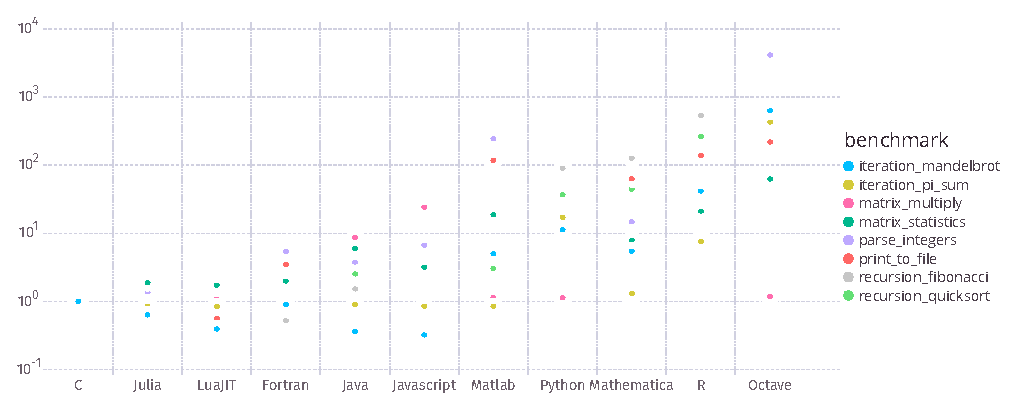
\includegraphics[width=.95\textwidth]{julia_benchmarks}
    \caption{Time benchmarks, relative to C, for various high-level languages}
    \label{fig:julia_benchmarks}
\end{figure}

The Julia developer community~\footnote{\url{https://github.com/JuliaLang/julia} [Accessed in
17/10/2017]} is very active, both in improving the standard library
and in developing separate packages, with over 1500 packages registered
in the language's official
repositories~\footnote{\url{https://pkg.julialang.org/} [Accessed in
17/10/2017]}, including NODAL.

Julia's high-performance, for a dynamic programming language, is attributed to
its type-inferred, Just-In-Time (JIT) compilation. Although a Julia program
can be written without type specifications, annotating variables with static
types is essential for performance.

\subsection{Parallel and Distributed Programming}
\label{sec:parallel-julia}

Julia's parallel and distributed programming model is based on message-passing
between processes. Each process has its own ID integer, and can run in a
separate processor core or machine. A Julia program does not manage multiple
processes, and is instead able to communicate using remote calls and
references, and data passed through channels.

Processes are launched and managed by cluster managers, which provide data
transport via TCP/IP in the built-in implementation. Cluster managers are also
able to manage the topology of the process network. NODAL currently uses the
built-in cluster manager, but studying the impact of different process
topologies might provide insight into improving NODAL's performance in
different distributed computing settings.

\subsubsection{Remote Calls \& References}

In Julia, a \textit{remote call} is a function call that is computed in a different
process. Remote calls can be made with the \texttt{remotecall} function
or macros from the \texttt{@spawn} family. The \texttt{remotecall} function
receives a regular function \texttt{f}, a process ID, and the arguments to
be passed to \texttt{f}. The \texttt{@spawn} macro receives an expression,
which can be a regular function call or any valid Julia expression, and
launches it in the next available Julia process.

Remote calls return immediately after launching the computation. The
results can be obtained using the \textit{remote reference} returned
by the remote call. Remote references are objects that reference data
stored in other processes, and can be of type \texttt{Future} or
\texttt{RemoteChannel}.

Figure~\ref{fig:remotecall_example} shows a code snippet that illustrates how
to use the \texttt{remotecall} function and the \texttt{@spawnat} macro. The
\texttt{@spawnat} macro receives as argument the target process in which to
launch the computation, in addition to a Julia expression. The Julia
interpreter can be launched with the \texttt{-p} argument, which receives an
integer and launches the correspondent number of Julia processes.

The code snippet in Figure~\ref{fig:remotecall_example} shows a remote call to
the \texttt{rand} function, to be launched in the process with ID 2. The other
arguments specify the 2 by 2 matrix that \texttt{rand} will fill with random
numbers. After this remote call the computation has been launched in a remote
process, and a \texttt{Future} is returned. The interpreter does not wait for
the computation to finish and goes back to wait for input.

\begin{figure}[htpb]
    \begin{minipage}{\linewidth}
    \begin{lstlisting}[language=C, basicstyle=\ttfamily\scriptsize,
        numbers=left,
        frame=no, showspaces=false, showstringspaces=false,
        numberstyle=\scriptsize,
        xleftmargin=1.5cm,
        keywords={%
            @spawnat, remotecall, Nullable, Any,
            fetch, Future, Array, Float64, julia%
        },
        otherkeywords={::, \&, \*, +, -, /, [, ], >, <}
    ]
$ ./julia -p 2

julia> r = remotecall(rand, 2, 2, 2)
Future(2, 1, 4, Nullable{Any}())

julia> s = @spawnat 2 1 .+ fetch(r)
Future(2, 1, 5, Nullable{Any}())

julia> fetch(s)
2x2 Array{Float64,2}:
 1.18526  1.50912
 1.16296  1.60607

    \end{lstlisting}
    %$
    \end{minipage}
    \caption{Using Julia's \texttt{remotecall} function and the \texttt{@spawnat} macro}
    \label{fig:remotecall_example}
\end{figure}

The call to the \texttt{@spawnat} macro in line 6 of
Figure~\ref{fig:remotecall_example} calls the \texttt{fetch} function. This
function receives a \texttt{Future} and blocks until the result is computed by
the remote process. The \texttt{.+} syntax represents an operation in an array.
In this case, the operation is summing 1 to every element of the matrix
returned by \texttt{fetch(r)}. The \texttt{@spawnat} macro also returns a
\texttt{Future}.  Finally, the call to \texttt{fetch} in line 9 of
Figure~\ref{fig:remotecall_example} gets the final value computed by the two
remote calls. The \texttt{remotecall\_fetch} function is a more efficient way
of launching a computation in a remote process and immediately asking for the
results, if there is no computation that can be performed while the process
waits.

A \texttt{Future} caches the remotely computed value after the first call,
and returns it without process communication in subsequent calls. A process
can only write once to a \texttt{Future}. If a more extended communication
is required, the programmer needs to use remote channels.

\subsubsection{Remote Channels}

Figure~\ref{fig:remotechannel_example} shows a more complex parallel and
distributed programming example using remote channels to manage a worker pool
that perform arbitrary jobs. Remote channels are created in a specific process,
but any process with a reference to a remote channel is able to write values to
it using the \texttt{put!} function, and read values from it using the
\texttt{take!} function. In remote channels from the standard library,
\texttt{put!} blocks until there is space in the channel and \texttt{take!}
blocks until there is a data object in the channel that can be taken, and
removes it from the channel when it completes.

\begin{figure}[htpb]
    \begin{minipage}{\linewidth}
    \begin{lstlisting}[language=C, basicstyle=\ttfamily\scriptsize,
        numbers=left,
        frame=no, showspaces=false, showstringspaces=false,
        numberstyle=\scriptsize,
        xleftmargin=1.5cm,
        keywords={%
            @spawnat, remotecall, Nullable, Any,
            fetch, Future, Array, Float64, julia,
            while, true, function, end, put!,
            take!, sleep, RemoteChannel, Channel,
            Int, Tuple, const, addprocs, @schedule,
            @everywhere, for, in, myid, @async,
            remote_do, workers%
        },
        otherkeywords={::, \&, \*, +, -, /, [, ], >, <, put!, take!}
    ]
julia> addprocs(4)

julia> const jobs = RemoteChannel(()->Channel{Int}(32))

julia> const results = RemoteChannel(()->Channel{Tuple}(32))

julia> @everywhere function do_work(jobs, results) # Defines method everywhere
       while true
           job_id = take!(jobs)
           exec_time = rand()
           sleep(exec_time) # Simulates time doing work
           put!(results, (job_id, exec_time, myid()))
       end
   end

julia> function make_jobs(n)
           for i in 1:n
               put!(jobs, i)
           end
       end

julia> n = 12

julia> @schedule make_jobs(n)

julia> for p in workers()
           @async remote_do(do_work, p, jobs, results)
       end

julia> while n > 0 # print out results
           job_id, exec_time, where = take!(results)
           n = n - 1
       end
    \end{lstlisting}
    %$
    \end{minipage}
    \caption{Using Julia's \texttt{RemoteChannel}}
    \label{fig:remotechannel_example}
\end{figure}

The snippet in Figure~\ref{fig:remotechannel_example} uses other macros and
functions. The \texttt{addprocs} function adds a specific number of processes
to the worker pool. The \texttt{@everywhere} macro is used to define data, or a
function, in all available Julia processes. The \texttt{@schedule} and
\texttt{@async} macros add asynchronous expressions to the Julia scheduler.
The \texttt{remote\_do} function launches a function in a given worker or
worker pool object.

NODAL uses remote calls and references to perform measurements, and remote
channels to manage the communication between search techniques and the user
program. The following section will describe NODAL's architecture and its
parallel and distributed implementation.

\section{Software Architecture}
\label{sec:nodal-arch}

Our main concern when developing NODAL was to ensure that search techniques
were independent from each other, making and managing their own requests for
measurements. To achieve this objective we developed a software architecture
that minimizes communication between processes and does not block on requests
to channels. NODAL uses non-blocking custom remote channels, the
\texttt{ResultChannel}.  The execution flow of search techniques is managed by
the techniques themselves, with a central control process that regularly polls
remote channels for results.

\begin{figure}[htpb]
    \centering
    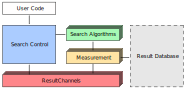
\includegraphics[width=.65\textwidth]{nodal_architecture}
    \caption{NODAL architecture, with a proposed database}
    \label{fig:nodal_architecture}
\end{figure}

Figure~\ref{fig:nodal_architecture} shows a high-level representation of
NODAL's architecture. User code that uses the library is responsible for
launching the main NODAL process, or \textit{tuning run}, and communicates with
it using remote channels. The NODAL main process is responsible to initialize
parallel and distributed search techniques using all processes available. Each
technique writes the best result it has found so far to its own remote channel.
The main process has references for all technique remote channels, and
periodically polls them for results.  After technique initialization there is
no blocking communication between the main process and search techniques, and
no communication between search techniques.

Search techniques are responsible for generating candidate configurations for
evaluation and requesting their measurement. This is done using remote calls to
the user-defined cost function. After measurement is complete, search
techniques write the current result to their remote channel.  The non-blocking
remote channel implementation used in NODAL  is described in
section~\ref{sec:nodal-measurement}.

Figure~\ref{fig:nodal_architecture} shows a grayed out database component,
which is not yet implemented. This database will shorten the time to obtain a
measurement of repeated configurations, and has the potential to be used to
train machine learning models or to give to the user knowledge about the search
space.

\subsection{Search and Measurement Call Graph}

A more detailed NODAL execution flow is presented in
Figure~\ref{fig:nodal_callgraph}. Each colored box represents a colored
component of Figure~\ref{fig:nodal_architecture}, and named smaller boxes
represent functions of each component. When necessary, a number marks the order
in which functions are called.

The entry point of a NODAL application is the user code, which calls the
\texttt{optimize} function. This is the main NODAL process, and must be
launched using a remote call. The main process initializes remote search
techniques using remote calls, by calling the
\texttt{initialize\_search\_tasks!} function. It is a non-enforced style of the
Julia language to append a ``\texttt{!}'' to functions that modify their
arguments. In this case, the modified argument is the list of remote channels
stored by the main process.  The initialization process is non-blocking, and it
returns after all techniques have been launched. The main process then enters a
loop, periodically checking for results from its remote channel references.

Initialized search techniques run their algorithms using search building
blocks, which are functions that perform some operation on the current
configuration of a search technique, measure it, and decide whether to accept
the new configuration. For example, the simulated annealing technique uses
the probabilistic improvement search building block.

\begin{figure}[htpb]
    \centering
    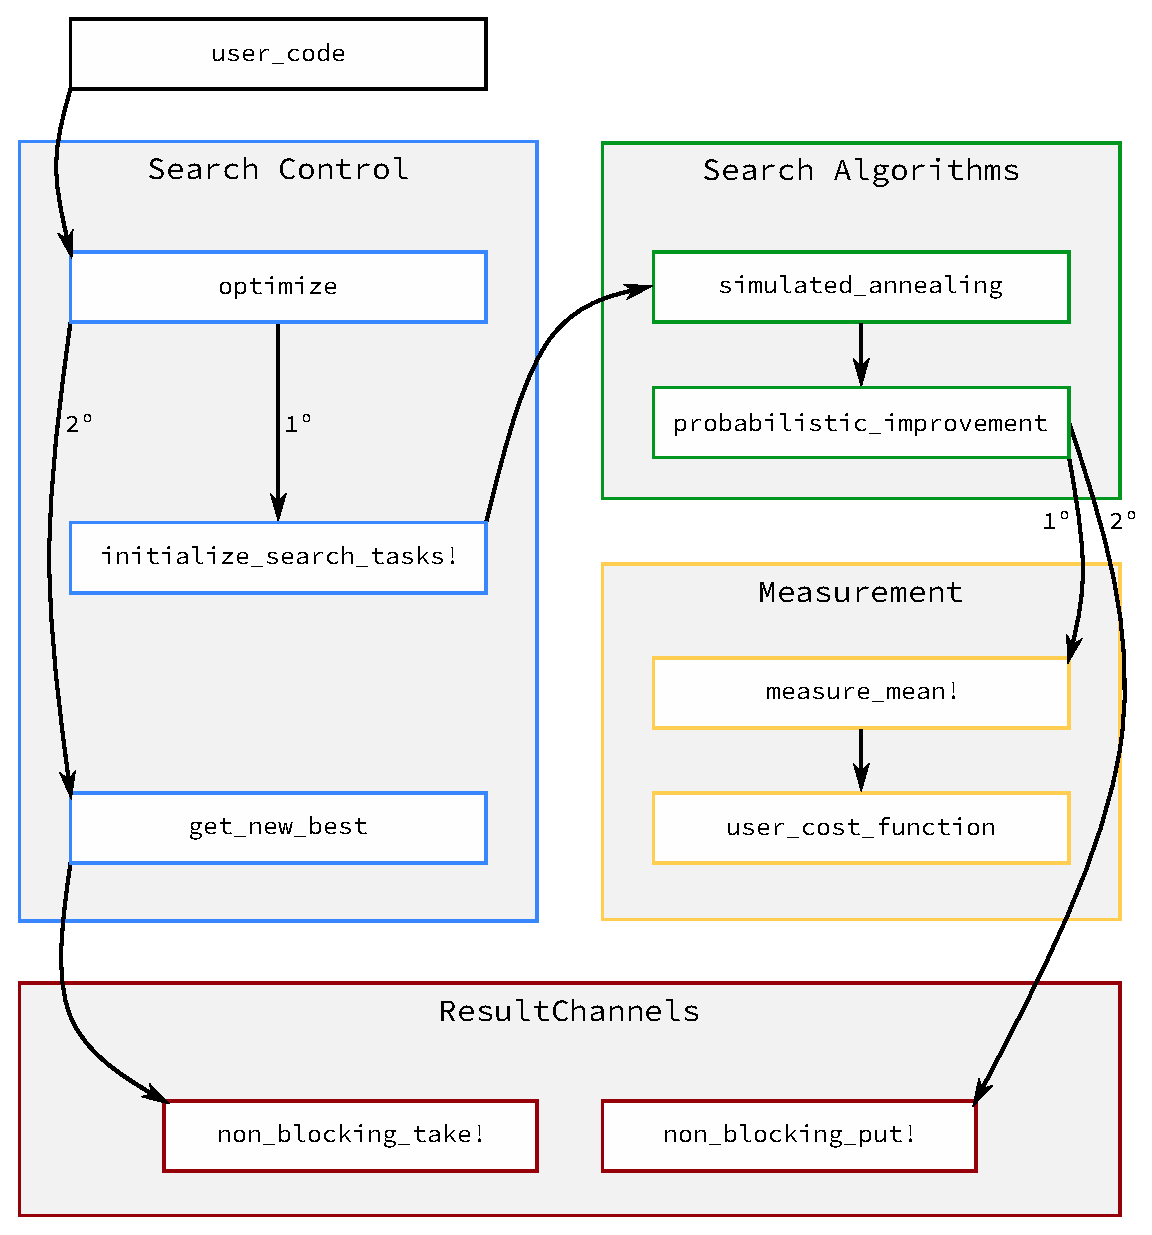
\includegraphics[width=.5\textwidth]{nodal_callgraph}
    \caption{NODAL search and measurement simplified call graph}
    \label{fig:nodal_callgraph}
\end{figure}

Search techniques request a measurement by performing remote calls to the
user-defined cost function. One way to do that is using the
\texttt{measure\_mean!} function, which perform multiple evaluations of a
function in parallel and returns the average of the measurements.  This is
useful for time measurements, for example, where fluctuations on the operating
system or system load can interfere with the results.

After a measurement is performed a search technique can update its algorithm
and immediately request another measurement.  Search techniques do not share
their best results so far, but this is an implementation choice and not an
architecture limitation.  We intend to implement a main process parameter that
can be set by the user and enable global result sharing in cases where may be
beneficial.  Scheduling of all remote calls performed in NODAL is performed by
Julia's scheduler. The next section describes the implementation of search
techniques and tools, and of measurement functions.

\section{Search \& Measurement Components}
\label{sec:nodal-components}

This section presents in more detail the search and measurement components,
discussing available parameters, search techniques, and measurement methods.

\subsection{Search}

The search space of an autotuner implemented using NODAL is defined as a
\texttt{Configuration} object that contains a set of \texttt{Parameter}
objects. Parameters are changed by search algorithms by using operator
functions specific to each parameter type. Currently, the only operator
available in NODAL is the neighbor operator, that randomizes a parameter's
value inside user-defined neighborhood. The ``radius'' of the neighborhood
can be changed on each call to the operator.

\subsubsection{Parameters}

Parameters are used to define performance-impacting program variables and their
limits. They can represent compiler flags, enumerations of algorithms that
solve a same problem, or numeric parameters of a program. Each parameter can be
set to an initial value or left unspecified, in which case it will be
randomized at the start of the search process.
Table~\ref{tab:nodal-parameters} shows the parameters currently implemented in
NODAL and the planned additions.

\begin{table}[htpb]
\centering
\begin{tabular}{@{}p{.15\textwidth}p{.15\textwidth}@{}}
\toprule
\textit{Implemented} & \textit{Planned} \\ \midrule
Boolean & Logarithmic \\
Float & Exponential \\
Integer & \\
Enumeration & \\
Permutation & \\ \bottomrule
\end{tabular}
\caption{NODAL implemented and planned parameters}
\label{tab:nodal-parameters}
\end{table}

\subsubsection{Search Building Blocks}

Search building blocks are responsible for generating a new candidate
configuration and launching parallel measurements for it. Search techniques can
use one or more building blocks to implement their algorithms. Building blocks
enable users to implement parallel and distributed search techniques without
having to write parallel code in Julia or becoming familiar with NODAL
specifics. Table~\ref{tab:nodal-blocks} shows the building blocks currently
implemented in NODAL and the planned additions.

\begin{table}[htpb]
\centering
\begin{tabular}{@{}p{.3\textwidth}p{.3\textwidth}@{}}
\toprule
\textit{Implemented} & \textit{Planned} \\ \midrule
First improvement & Best Improvement \\
Probabilistic Improvement & \\
Greedy Construction & \\
Random Walk & \\ \bottomrule
\end{tabular}
\caption{NODAL implemented and planned search building blocks}
\label{tab:nodal-blocks}
\end{table}

\subsubsection{Search Techniques}

\begin{table}[htpb]
\centering
\begin{tabular}{@{}p{.4\textwidth}p{.35\textwidth}@{}}
\toprule
\textit{Implemented} & \textit{Planned} \\ \midrule
Iterative First Improvement & Iterative Best Improvement \\
Iterative Greedy Construction & Randomized Best Improvement \\
Iterative Probabilistic Improvement & Randomized Best Improvement \\
Randomized First Improvement & Iterative Best Construction \\
Simulated Annealing & Dynamic Local Search \\
Iterated Local Search & Tabu Search \\
 & Ant Colony Optimization \\
 & Particle Swarm Optimization \\
 & Nelder-Mead \\
 & Genetic Algorithms \\ \bottomrule
\end{tabular}
\caption{NODAL implemented and planned search techniques}
\label{my-label}
\end{table}

\begin{figure}[htpb]
    \begin{minipage}{\linewidth}
    \begin{lstlisting}[language=C, basicstyle=\ttfamily\scriptsize,
        numbers=left,
        frame=no, showspaces=false, showstringspaces=false,
        numberstyle=\scriptsize,
        xleftmargin=1.5cm,
        keywords={%
            @spawnat, remotecall, Nullable, Any,
            @fetch, Future, Array, Float64, julia,
            while, true, function, end, put!,
            take!, sleep, RemoteChannel, Channel,
            Int, Tuple, const, addprocs, @schedule,
            @everywhere, for, in, myid, @async,
            remote_do, workers, Result, Real,
            AbstractFloat, deepcopy, rand, exp, true,
            Function, false, Run, return%
        },
        otherkeywords={::, \&, \*, +, -, /, [, ], >, <, put!, take!, neighbor!,
                       update!}
    ]
function simulated_annealing(tuning_run::Run,
                             channel::RemoteChannel;
                             temperature::Function = log_temperature)
    iteration = 1

    function iterate(tuning_run::Run)
        p          = temperature(iteration)
        iteration += 1
        return probabilistic_improvement(tuning_run, threshold = p)
    end

    technique(tuning_run,
              channel,
              iterate,
              name = "Simulated Annealing")
end
    \end{lstlisting}
    %$
    \end{minipage}
    \caption{The simulated annealing search technique}
    \label{fig:simulated annealing}
\end{figure}

\subsubsection{Parallel and Distributed Search}

\subsection{Measurement}
\label{sec:nodal-measurement}

\subsubsection{Result Remote Channels}

\begin{figure}[htpb]
    \begin{minipage}{\linewidth}
    \begin{lstlisting}[language=C, basicstyle=\ttfamily\scriptsize,
        numbers=left,
        frame=no, showspaces=false, showstringspaces=false,
        numberstyle=\scriptsize,
        xleftmargin=1.5cm,
        keywords={%
            @spawnat, remotecall, Nullable, Any,
            @fetch, Future, Array, Float64, julia,
            while, true, function, end, put!,
            take!, sleep, RemoteChannel, Channel,
            Int, Tuple, const, addprocs, @schedule,
            @everywhere, for, in, myid, @async,
            remote_do, workers, Result, Real,
            AbstractFloat, deepcopy, rand, exp, true,
            Function, false, Run, mutable, struct,
            ResultChannel, AbstractChannel, return%
        },
        otherkeywords={::, \&, \*, +, -, /, [, ], >, <, put!, take!, neighbor!,
                       update!}
    ]
mutable struct ResultChannel <: AbstractChannel
    current_result::Result
    ResultChannel(result::Result) = new(result)
end

function put!(channel::ResultChannel, result::Result)
    if result.cost_minimum < channel.current_result.cost_minimum
        channel.current_result = result
    end
    channel
end

function take!(channel::ResultChannel)
    fetch(channel)
end

function fetch(channel::ResultChannel)
    channel.current_result
end
    \end{lstlisting}
    %$
    \end{minipage}
    \caption{\texttt{ResultChannel} Implementation}
    \label{fig:resultchannel}
\end{figure}

\subsubsection{Parallel and Distributed Measurement}

\begin{figure}[htpb]
    \begin{minipage}{\linewidth}
    \begin{lstlisting}[language=C, basicstyle=\ttfamily\scriptsize,
        numbers=left,
        frame=no, showspaces=false, showstringspaces=false,
        numberstyle=\scriptsize,
        xleftmargin=1.5cm,
        keywords={%
            @spawnat, remotecall, Nullable, Any,
            @fetch, Future, Array, Float64, julia,
            while, true, function, end, put!,
            take!, sleep, RemoteChannel, Channel,
            Int, Tuple, const, addprocs, @schedule,
            @everywhere, for, in, myid, @async,
            remote_do, workers, Result, Real,
            AbstractFloat, deepcopy, rand, exp, true,
            Function, false, Run, Array, Configuration,
            pmap, mean, return%
        },
        otherkeywords={::, \&, \*, +, -, /, [, ], >, <, put!, take!, neighbor!,
                       update!}
    ]
function measure_mean!(tuning_run::Run, x::Configuration)
    configurations = Array{Configuration}(tuning_run.cost_evaluations)
    fill!(configurations, deepcopy(x))

    pmap_cost(x::Configuration) = tuning_run.cost(x, tuning_run.cost_arguments)
    results = pmap(pmap_cost, configurations)

    for i = 1:tuning_run.cost_evaluations
        tuning_run.cost_values[i] = results[i]
    end

    mean(results)
end

function sequential_measure_mean!(tuning_run::Run, x::Configuration)
    for i = 1:tuning_run.cost_evaluations
        tuning_run.cost_values[i] = tuning_run.cost(x, tuning_run.cost_arguments)
    end
    mean(tuning_run.cost_values)
end
    \end{lstlisting}
    %$
    \end{minipage}
    \caption{Parallel and distributed measurement functions}
    \label{fig:measurement}
\end{figure}

\section{Examples}
\label{sec:nodal-examples}

\subsection{A Tool for Compiler Autotuning}
\label{sec:nodal-gpu-tuner}

\subsection{Travelling Salesperson Problem}
\label{sec:tsp}

\section{Summary}
\label{sec:concl}
